The main function of the system is to allow users to make a request or a reservation for a taxi and taxi drivers to take care of a specific request.
This is a list of the main actions that our system will provide:

\begin{itemize}
    \item Users:
        \begin{itemize}
        	\item Sign up into the system.
        	\item Log into the system.
        	\item Request a taxi.
        	\item Reserve a taxi.
        	\item Delete requests or reservations.
        	\item Visualize information about requests or reservations.
        	\item Manage their account.
        \end{itemize}
    \item Taxi drivers:
        \begin{itemize}
        	\item Sign up into the system.
        	\item Log into the system.
        	\item Receive information from the system about the city's area they have to cover.
        	\item Notify the system of their availability.
        	\item Receive requests and reservations from the system.
        	\item Accept or decline requests.
        	\item Manage their account.
        \end{itemize}
\end{itemize}

\newpage
\subsubsection{Use Case diagram}
From the list of actions described above, we can derive a Use Case Diagram of our system.

\begin{figure}[h]
    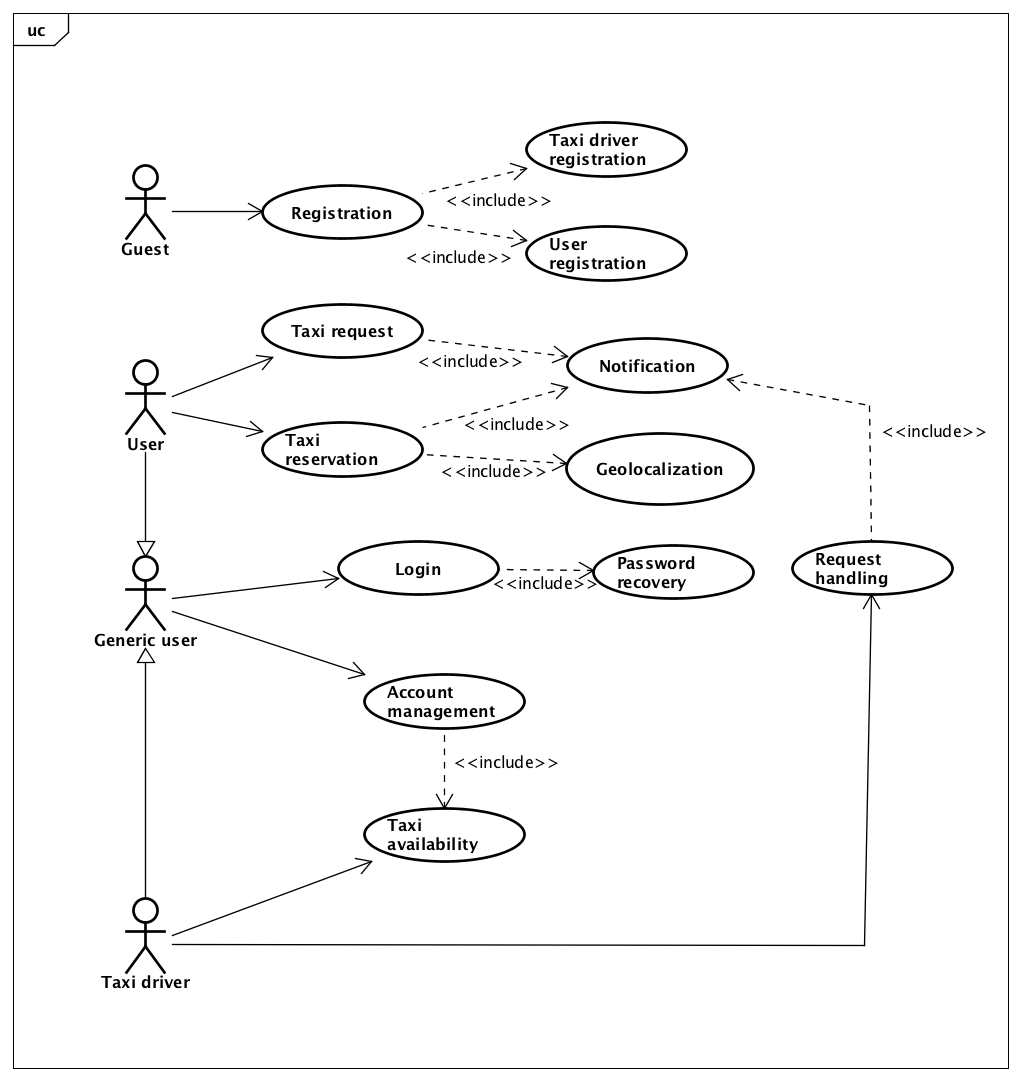
\includegraphics[width=11cm]{./Diagrams/UseCaseDiagram.png}
    \caption{Use Case diagram}
    \centering
\end{figure}

 